\section{Metodologia Applicata}
\label{sec:methodology}
\subsection{Workflow}
\begin{figure}[hbpt!]
		\centering
		\includesvg[inkscapelatex=false, width=0.7\textwidth]{images/workflow}
  		\caption{Il workflow del nostro metodo (ripreso da \cite{lyu2018deep})}
        \label{fig:workflow}
\end{figure}
Il workflow del nostro metodo ricalca in buona parte quello di \cite{lyu2018deep} ed è mostrato in 
Figura \ref{fig:workflow}: 
\begin{enumerate}
    \item Unione dei dati grezzi per ottenere i dataset su cui operare (tale passo non è riportato nella Figura 
          \ref{fig:workflow} in quanto è stato utilizzato solo per il test binario e il test ternario e dunque
          non viene effettuato in quello che è il test principale di questo lavoro).
    \item Preprocessing sui dati che rappresentano le espressioni genetiche di vari genomi.
    \item Classificazione delle varie tipologie di tumori tramite l'uso di una rete neurale convoluzionale. 
    \item Valutazione delle performance della rete neurale. 
    \item Generare le heatmap per ogni classe tumorale e selezionare i geni corrispondenti ai pixel 
          con la massima intensità.
    \item Convalidare i percorsi biologici dei geni selezionati.
\end{enumerate}

\subsection{Dati utilizzati}
Sono stati utilizzati i \textbf{normalized-level3 RNA-Seq gene expression} data di 33 tipi di tumore presenti 
nel Pan-Cancer Atlas. Un elenco dettagliato di tutti i 33 tipi di tumore e del corrispondente numero di campioni è
riportato nella Tabella \ref{tab:tumor-samples} a pagina \pageref{tab:tumor-samples}. 
I dati contengono 10.267 campioni di tumore su 20.531 campioni totali. I dati sono stati scaricati 
da \textit{Firehose}\cite{firehose}, che è un tool sviluppato dal TGCA network e gestito dal Broad Institute.
\textit{Firehose} è "una serie di tool e pipeline sviluppati per processare ed analizzare vari tipi di dati genomici 
e proteici su vasta scala" \cite{tgcatools}.

Per il caso binario (DLBC e UCS) e per il caso ternario (BLCA, CESC e LGG) abbiamo ricreato il dataset di partenza 
unendo i raw data delle classi prese in esame, abbiamo effettuato data cleaning sui dati in quanto erano presenti 
dei sample non appartenenti al tessuto tumorale e abbiamo aggiunto le label per distinguere le classi. 
Per il caso generale, invece, abbiamo deciso di utilizzare il dataset messo a disposizione da \cite{lyu2018deep} 
che è stato creato a partire dagli stessi dati.

% Tabella: Numero di campioni di RNA-Sequence Tumorali
\begin{table}[htbp]
    \centering 
    \caption{Numero campioni di RNA-Sequence tumorali.}
    \large{
    \begin{tabular}{llr}
    \toprule
    Classe   & Coorte & Numero    \\
    tumorale &        & Campioni  \\
    \midrule
    Adrenocortical carcinoma                        & ACC  & $79$   \\
    Bladder urothelial carcinoma                    & BLCA & $408$  \\
    Breast invasive carcinoma                       & BRCA & $1093$ \\
    Cervical and endocervical cancers               & CESC & $304$  \\
    Cholangiocarcinoma                              & CHOL & $36$   \\
    Colon adenocarcinoma                            & COAD & $457$  \\
    Lymphoid Neoplasm Diffuse Large B-cell Lymphoma & DLBC & $48$   \\
    Esophageal carcinom                             & ESCA & $184$  \\
    Glioblastoma multiforme                         & GBM  & $160$  \\
    Head and Neck squamous cell carcinoma           & HNSC & $520$  \\
    Kidney Chromophobe                              & KICH & $66$   \\
    Kidney renal clear cell carcinoma               & KIRC & $533$  \\
    Kidney renal papillary cell carcinoma           & KIRP & $290$  \\
    Acute Myeloid Leukemia                          & LAML & $179$  \\
    Brain Lower Grade Glioma                        & LGG  & $516$  \\
    Liver hepatocellular carcinoma                  & LIHC & $371$  \\
    Lung adenocarcinoma                             & LUAD & $515$  \\
    Lung squamous cell carcinoma                    & LUSC & $501$  \\
    Mesothelioma                                    & MESO & $87$   \\
    Ovarian serous cystadenocarcinoma               & OV   & $304$  \\
    Pancreatic adenocarcinoma                       & PAAD & $178$  \\
    Pheochromocytoma and Paraganglioma              & PCPG & $179$  \\
    Prostate adenocarcinoma                         & PRAD & $497$  \\
    Rectum adenocarcinoma                           & READ & $166$  \\ 
    Sarcoma                                         & SARC & $259$  \\ 
    Skin Cutaneous Melanoma                         & SKCM & $469$  \\ 
    Stomach adenocarcinoma                          & STAD & $415$  \\ 
    Testicular Germ Cell Tumors                     & TGCT & $150$  \\ 
    Thyroid carcinoma                               & THCA & $501$  \\ 
    Thymoma                                         & THYM & $120$  \\ 
    Uterine Corpus Endometrial Carcinoma            & UCEC & $545$  \\ 
    Uterine Carcinosarcoma                          & UCS  & $57$   \\ 
    Uveal Melanoma                                  & UVM  & $80$   \\ 
    \midrule
    \textbf{Totale campioni}                        &      & $\mathbf{10267}$  \\
    \bottomrule
    \label{tab:tumor-samples}
    \end{tabular} 
    } % end large
\end{table}

\subsubsection{RSEM: RNA-Seq Expetation Maximization}~\newline
I dati utilizzati nell'ambito di questo progetto sono stati ottenuti dal FireHose Broad GDAC\footnote{Con sede a
Cambridge, nel Massachusetts, il Broad Institute è stato fondato nel 2004 per realizzare la promessa della medicina
genomica, tre anni dopo il completamento del Progetto Genoma Umano, che gli scienziati del Broad hanno contribuito a
creare e guidare. Le nostre origini sono radicate nella genomica e, dal 2004, la ricerca biomedica e la conoscenza si
sono ampliate, così come noi. I nostri ricercatori sono profondamente collaborativi, lanciano agilmente progetti
innovativi e ad alto rischio su ogni scala, acquisiscono conoscenze sui meccanismi biologici delle malattie, inventano
nuove tecnologie, costruiscono e implementano strumenti computazionali, sviluppano nuove terapie da portare in clinica,
fanno da tutor e formano la prossima generazione di scienziati oltre che condividere apertamente i dati e gli
strumenti per consentire progressi in ogni settore della società.}.
Questi ultimi sono ottenuti dall'applicazione di un software denominato RSEM \cite{li2011rsem} così definito: 
RSEM è un pacchetto software di facile utilizzo per quantificare le abbondanze di geni e isoforme da dati RNA-Seq 
single-end o paired-end. RSEM, inoltre, è stato progettato per lavorare con letture allineate a sequenze di trascritti,
anziché a letture allineate a sequenze di genomi interi. 
L'utilizzo di allineamenti a livello di trascrizione ha come vantaggio quello di consentire facilmente l'analisi di
campioni di specie senza genomi sequenziati ma con un trascrittoma decentemente caratterizzato (magari attraverso
l'assemblaggio del trascrittoma RNA-Seq \cite{robertson2010novo, grabherr2011full}). 
Infine, la lunghezza totale di tutti i possibili trascritti è spesso molto inferiore alla lunghezza del genoma,
consentendo un allineamento più rapido a livello di trascritto.
RSEM produce stime di abbondanza, intervalli di credibilità al 95\%, file di visualizzazione, può anche simulare i dati
RNA-Seq, e a differenza di altri strumenti esistenti, il software non richiede un genoma di riferimento. Pertanto, in
combinazione con un assemblatore di trascrittomi de novo, RSEM consente una quantificazione accurata dei trascritti 
per le specie prive di genomi sequenziati. Su set di dati simulati e reali, RSEM ha prestazioni superiori o paragonabili
ai metodi di quantificazione che si basano su un genoma di riferimento. Sfruttando la capacità di RSEM di
utilizzare efficacemente le letture a mappatura ambigua, è stato dimostrato che le stime accurate dell'abbondanza a
livello genico si ottengono al meglio con un gran numero di short read single-end. D'altra parte, le stime delle
frequenze relative delle isoforme all'interno di singoli geni possono essere migliorate con l'uso di letture 
paired-end, a seconda del numero di possibili forme di splice per ciascun gene. Inoltre RSEM possiede diversi
allineatori di sequenze genomiche come Bowtie, Bowtie2 e STAR. Gli input di tali strumenti risultano quindi essere le
sequenze di RNA prodotte dalla piattaforma genomica Illumina sottoforma di file formato fasta o fastaq. Oltre a ciò,
viene dato anche un file contente l'annotazione genetica che RSEM userà come rifermento per stimare il gene expression 
level. 
% Parte ML / statistica di RSEM 
Dopo l'allineamento delle read tramite uno degli algoritmi sopra citati, RSEM calcola le stime di abbondanza ML
utilizzando l'algoritmo Expectation-Maximization (EM) per il suo modello statistico. Sono disponibili diverse opzioni
per specificare il modello utilizzato da RSEM, che deve essere personalizzato in base al protocollo RNA-Seq che ha
prodotto le letture in ingresso. Ad esempio, se viene utilizzato un protocollo specifico per ogni filamento, è
necessario specificare l'opzione \texttt{--strand-specific}. Altrimenti, si presume che una lettura abbia la stessa
probabilità di provenire dalla direzione \textit{senso} o \textit{antisenso}. L'output principale di RSEM consiste 
di due file: uno per le stime a livello di isoforma e l'altro per le stime a livello di gene. 
Le stime di abbondanza sono fornite in termini di due misure. La prima è una stima del numero di frammenti derivati 
da una determinata isoforma o gene. La seconda, è la frazione stimata di trascritti costituita da una determinata
isoforma o gene. Questa misura può essere utilizzata direttamente come valore compreso tra zero e uno o può essere
moltiplicata per $10^6$ per ottenere una misura in termini di trascritti per milione (TPM). 

\subsection{Fase di Preprocessing}
I dati contengono il conteggio normalizzato delle read per ogni gene, ma l'intervallo dei valori è enorme e alcuni
alcuni valori sono più piccoli di 1.
Perciò, come \cite{lyu2018deep}, abbiamo applicato prima una trasformazione usando $y = \log_2 (x + 1)$ per ridurre la
scala. Poi abbiamo posto a 0 tutti i valori inferiori a 1, poiché è molto probabile che si tratti di rumore.
Successivamente, abbiamo confrontato i geni con un file di annotazione (aggiornato al 03 aprile 2018) scaricato
dall'NCBI. Circa 1000 geni non sono stati trovati nel file di annotazione, quindi sono stati rimossi. 
Abbiamo poi utilizzato una soglia di varianza pari a $1,19$ per filtrare i geni i cui livelli di espressione 
rimangono quasi invariati tra i campioni. Il numero di geni è stato così ulteriormente ridotto a $10.381$. 
Questa soglia è stata scelta considerando sia l'accuratezza della classificazione sia l'integrità
dell'insieme di geni. Una soglia più alta ridurrà maggiormente le "weak feature", in modo da migliorare l'accuratezza
della classificazione. Una soglia più bassa, invece, permette di mantenere un maggior numero di geni, in modo da 
non perdere i reali biomarker specifici del gene. Inoltre, per comodità nella fase successiva, abbiamo voluto che il
numero di geni filtrati fosse vicino a un numero quadrato.
Per dare in pasto i dati alla rete neurale convoluzionale, essi sono stati incorporati in immagini 2D. I primi geni 
sono ordinati in base al numero di cromosoma, perché è più probabile che geni adiacenti interagiscano tra loro. 
Poi i dati sono stati rimodellati da una matrice $10.381 \times 1$ in un'immagine $102 \times 102$ aggiungendo 
alcuni zeri all'ultima riga dell'immagine. Quindi tutte le immagini vengono normalizzate per assicurarsi che
che l'intervallo sia $[0, 255]$. Le immagini generate delle diverse classi sono mostrate nella Figura
\ref{fig:img2Dexample} a pagina \pageref{fig:img2Dexample}.
	\begin{figure}[h!]
		\centering
		% prima riga
		\subfloat[][ACC]{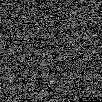
\includegraphics[scale=0.3]{images/tumorimg/ACC}}   \hfill % 1
		\subfloat[][BLCA]{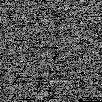
\includegraphics[scale=0.3]{images/tumorimg/BLCA}} \hfill % 2
		\subfloat[][BRCA]{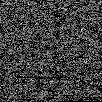
\includegraphics[scale=0.3]{images/tumorimg/BRCA}} \hfill % 3
		\subfloat[][CESC]{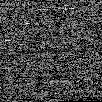
\includegraphics[scale=0.3]{images/tumorimg/CESC}} \hfill % 4
		\subfloat[][CHOL]{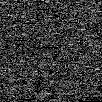
\includegraphics[scale=0.3]{images/tumorimg/CHOL}} \hfill % 5
		\subfloat[][COAD]{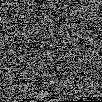
\includegraphics[scale=0.3]{images/tumorimg/COAD}} \hfill % 6
		\subfloat[][DLBC]{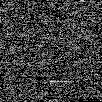
\includegraphics[scale=0.3]{images/tumorimg/DLBC}} \hfill % 7
		\subfloat[][ESCA]{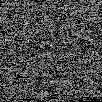
\includegraphics[scale=0.3]{images/tumorimg/ESCA}} \hfill % 8
		\subfloat[][GBM]{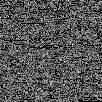
\includegraphics[scale=0.3]{images/tumorimg/GBM}}   \hfill % 9
		\subfloat[][HNSC]{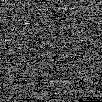
\includegraphics[scale=0.3]{images/tumorimg/HNSC}} \hfill % 10
		\subfloat[][KICH]{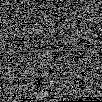
\includegraphics[scale=0.3]{images/tumorimg/KICH}} \\     % 11
		% seconda riga
		\subfloat[][KIRC]{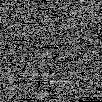
\includegraphics[scale=0.3]{images/tumorimg/KIRC}} \hfill % 12
		\subfloat[][KIRP]{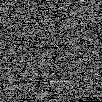
\includegraphics[scale=0.3]{images/tumorimg/KIRP}} \hfill % 13
		\subfloat[][LAML]{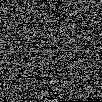
\includegraphics[scale=0.3]{images/tumorimg/LAML}} \hfill % 14
		\subfloat[][LGG]{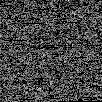
\includegraphics[scale=0.3]{images/tumorimg/LGG}}   \hfill % 15
		\subfloat[][LIHC]{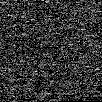
\includegraphics[scale=0.3]{images/tumorimg/LIHC}} \hfill % 16
		\subfloat[][LUAD]{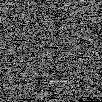
\includegraphics[scale=0.3]{images/tumorimg/LUAD}} \hfill % 17
		\subfloat[][LUSC]{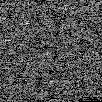
\includegraphics[scale=0.3]{images/tumorimg/LUSC}} \hfill % 18
		\subfloat[][MESO]{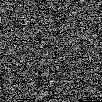
\includegraphics[scale=0.3]{images/tumorimg/MESO}} \hfill % 19
		\subfloat[][OV]{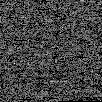
\includegraphics[scale=0.3]{images/tumorimg/OV}}     \hfill % 20
		\subfloat[][PAAD]{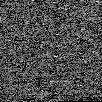
\includegraphics[scale=0.3]{images/tumorimg/PAAD}} \hfill % 21
		\subfloat[][PCPG]{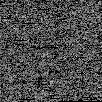
\includegraphics[scale=0.3]{images/tumorimg/PCPG}} \\ % 22
		% terza riga
		\subfloat[][PRAD]{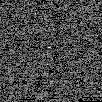
\includegraphics[scale=0.3]{images/tumorimg/PRAD}} \hfill % 23
		\subfloat[][READ]{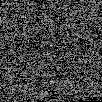
\includegraphics[scale=0.3]{images/tumorimg/READ}} \hfill % 24
		\subfloat[][SARC]{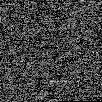
\includegraphics[scale=0.3]{images/tumorimg/SARC}} \hfill % 25
		\subfloat[][SKCM]{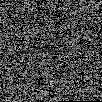
\includegraphics[scale=0.3]{images/tumorimg/SKCM}} \hfill % 26
		\subfloat[][STAD]{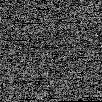
\includegraphics[scale=0.3]{images/tumorimg/STAD}} \hfill % 27
		\subfloat[][TGCT]{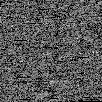
\includegraphics[scale=0.3]{images/tumorimg/TGCT}} \hfill % 28
		\subfloat[][THCA]{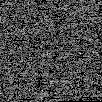
\includegraphics[scale=0.3]{images/tumorimg/THCA}} \hfill % 29
		\subfloat[][THYM]{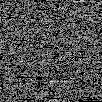
\includegraphics[scale=0.3]{images/tumorimg/THYM}} \hfill % 30
		\subfloat[][UCEC]{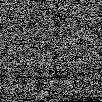
\includegraphics[scale=0.3]{images/tumorimg/UCEC}} \hfill % 31
		\subfloat[][UCS]{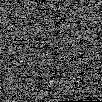
\includegraphics[scale=0.3]{images/tumorimg/UCS}}   \hfill % 32
		\subfloat[][UVM]{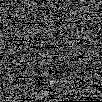
\includegraphics[scale=0.3]{images/tumorimg/UVM}}   \hfill % 33
		\caption{Un esempio di immagini 2D incorporate dalla classe 1 alla classe 33.}
		\label{fig:img2Dexample}
	\end{figure}

\subsection{Classificazione delle immagini tramite Neural Network}
\label{methology_sec:ClassNN}
\begin{figure}[h!]
		\centering
		\includesvg[inkscapelatex=false, width=1.1\textwidth]{images/CNN}
  		\caption{L'architettura della rete neurale convoluzionale}
        \label{fig:cnn}
\end{figure}
A causa dello squilibrio nel set di dati, alcune classi hanno pochi campioni, quindi la rete neurale non dovrebbe
contenere troppi strati al fine di evitare un grave overfitting. 
Alla fine abbiamo utilizzato la rete neurale convoluzionale di \cite{lyu2018deep} composta da tre layer convoluzionali 
e tre layer completamente connessi, come mostrato in Figura \ref{fig:cnn}. Il primo layer convoluzionale "conv1"
contiene 64 filtri diversi, mentre il secondo e il terzo layer convoluzionale contengono rispettivamente 128 e 256
filtri. Il layer di max-pooling e il layer di batch normalization sono posti immediatamente dopo
ogni layer convoluzionale. Prima di entrare nel layer fully-connected viene aggiunto un layer di drop-out, il cui 
tasso di drop-out è del 25\%. Le dimensioni dei tre layer fully-connected sono 36.864, 1.024 e 512 rispettivamente.
Abbiamo scelto la Cross Entropy come funzione di perdita e l'ottimizzatore Adam per aggiornare i pesi. 
Abbiamo utilizzato la 10 fold cross validation per addestrare la rete neurale convoluzionale e testarne le
prestazioni. \newline

\subsubsection{Convolutional Neural Network}~\newline
\label{subsubsec:3.4.1}
La CNN è una rete neurale feedforward che è in grado di estrarre caratteristiche dai dati, tramite connessioni locali e 
un pattern di pesi replicati in ogni layer nascosto della rete. Questo pattern è definito kernel ed il processo di 
applicazione del kernel sull'input è detto convoluzione. 
Diversamente dai metodi classici di estrazione delle caratteristiche \cite{1717463, lindeberg2012scale}, le CNN non 
hanno bisogno di estrarre caratteristiche manualmente. L'architettura della CNN si ispira alla percezione visiva
\cite{hubel1962receptive}, quindi imita il funzionamento del sistema oculare umano. In questa visione possiamo 
entrare nel dettaglio di questa struttura, affermando che un neurone biologico del cervello che fa da feedback 
alla corteccia visiva può corrispondere ad un neurone artificiale che compone uno strato della rete; i layer che
applicano la convoluzione usano i kernel che fungono da recettori e possono catturare varie caratteristiche della
realtà; le funzioni di attivazione possono simulare il funzionamento di trasmissione tra vari gruppi di neuroni,
imponendo che solo i segnali elettrici neurali, superiori ad una certa soglia, possono essere trasmessi al gruppo
successivo o al singolo neurone. Le funzioni di perdita e gli ottimizzatori sono strumenti che permettono al
sistema CNN di imparare e migliorarsi per raggiungere gli obiettivi che ci aspettiamo. 
\begin{figure}[hbpt!]
		\centering
		\includesvg[inkscapelatex=false, width=\textwidth]{images/cl_vs_fcl} %CNNvsFC
  		\caption{Confronto architterture CNN e FC \cite{9451544}}
        \label{fig:cnnvsfc}
\end{figure}
Rispetto al layer fully connected (FC), come in Figura \ref{fig:cnnvsfc}, le CNN possiedono molti vantaggi:
\begin{enumerate}
    \item \textbf{Connessioni locali:} Ogni neurone non è più collegato a tutti i neuroni del layer precedente, 
          ma solo ad un piccolo numero di neuroni. Ciò è utile a ridurre i parametri ed accelerare la 
          convergenza del modello. 
    \item \textbf{Ripartizione del peso:} un gruppo di connessioni possono condividere gli stessi pesi e ciò riduce
          ulteriormente i parametri.
    \item \textbf{Riduzione della dimensione di downsampling:} il principio della correlazione locale dell'immagine
          applicata dall'operazione di convoluzione serve a filtrare la dimensione dell'immagine (downsample
          dell'immagine) conservando le informazioni più complesse che devono essere processate da uno strato 
          più profondo. Il downsample rimuove anche le caratteristiche banali consentendo al modello di
          avere un minor numero di parametri negli strati più profondi. 
\end{enumerate}
Queste tre caratteristiche accattivanti rendono le CNN uno degli algoritmi più rappresentativi nel campo del deep
learning. Il termine "convoluzione" si riferisce ad un processo matematico lineare tra matrici. 
I layer convoluzionali, non lineari, di pooling e fully connected sono solo alcuni tra i molti layer che compongono 
una CNN. Nei layer di una CNN si fa distinzione tra layer con parametri e layer senza parametri. 
I layer con parametri sono quelli convoluzionali e quelli fully connected. Quelli senza parametri sono i layer 
di pooling e i layer non lineari. Nel sottoparagrafo seguente analizzeremo come agiscono i differenti layer durante 
la classificazione effettuata con una CNN.


\subsubsection{Convolutional Neural Network Layers}~\newline
Le CNN sono composte da vari strati che hanno la capacità di comporre l'input tramite l'uso di funzioni non lineari e 
di associarlo ad una target class.
I principali componenti base per la costruzione di una CNN sono:
\begin{description}
    \item[Convolutional layer] Il layer di convoluzione è il layer più semplice ma allo stesso tempo più 
    importante di una CNN.
    Fondamentalmente applica il kernel oppure moltiplica o la matrice dei pixel generata per l'immagine o 
    l'oggetto dato in input per produrre una mappa di attivazione per l'immagine fornita. Il vantaggio 
    principale della mappa di attivazione è che memorizza tutte le caratteristiche distintive di una data 
    immagine riducendo allo stesso tempo la quantità di dati da elaborare.
    La matrice con cui i dati sono convogliati è un rilevatore di caratteristiche che fondamentalmente è un 
    insieme di valori con cui la rete è compatibile.
    Diverse versioni dell'immagine vengono generate utilizzando diversi valori del rilevatore di funzionalità.
    Inoltre il modello CNN è anche addestrato con backpropagation per accertare l'errore minimo in ogni layer e,
    a seconda dell'errore più basso ottenuto dal layer, si imposta la profondità, ossia il numero di filtri, e 
    il padding.
    La Figura \ref{fig:ConvKernel} mostra come funziona la convoluzione. 
    Questo passaggio comporta la convoluzione della matrice contenente i dati dell'immagine e quindi il 
    rilevatore di caratteristiche che ci dà una mappa di attivazione o una mappa caratteristica. 
    Ciò che accade nella convoluzione è che i valori su posizioni identiche nei dati e nella mappa delle
    caratteristiche, cioè i valori che hanno valore 1 o più di 1, vengono mantenuti mentre il resto viene rimosso.
    La matrice dei dati dell'immagine viene confrontata $3 \times 3$ alla volta. 
    La dimensione del rilevatore di caratteristiche varia a seconda del tipo di CNN utilizzato. 
    Per esempio ci sono versioni di CNN che utilizzano filtri $5 \times 5$ o anche filtri in scala $7 \times 7$. 
    La convoluzione segue la seguente formula: 
    \[
        (f ^{\ast} g)(t) = \int_{-\infty}^{\infty} f(\beta)\,g\,(t - \beta)\,d \beta
    \]
    che mira a mostrare come una funzione modifica la forma dell'altra. Nell'immagine \ref{fig:ConvLayer} 
    si nota che i dati generati per questa immagine sono stati modificati usando il filtro per generare la 
    mappa di attivazione. 
    L'insieme di tutte le feature map create con vari filtri formano un livello di convoluzione. Altri fattori 
    che influiscono sulla potenzialità di un strato convoluzionale sono lo \textbf{Stride} e il \textbf{Padding}:
    \begin{description}
        \item[Stride] In realtà, per le CNN esistono altre possibilità per diminuire ulteriormente i parametri
        in un layer convoluzionale, impedendo anche effetti collaterali dovuti a questa diminuzione. Una di
        queste opzioni è lo stride. Si assume per semplicità questa ipotesi di base che afferma che il nodo del
        livello successivo abbia molte sovrapposizioni con i suoi vicini quando guardano le regioni di una
        immagine. Possiamo manipolare queste sovrapposizione tra i campi recettivi che compongono un layer
        convoluzionale gestendo lo stride. La Figura \ref{fig:Stride}, è un esempio che inizia con una data
        immagine $7\times 7$. Se spostiamo il filtro un nodo alla volta, possiamo avere solo un'uscita 
        $5 \times 5$. Si noti che l'uscita delle tre matrici di sinistra in Figura \ref{fig:Stride}, hanno 
        una sovrapposizione (un totale di tre tra quelle centrali e di tre tra quelle di destra). Tuttavia, 
        se ci muoviamo e facciamo ogni movimento con stride 2, allora l'uscita sarà $3 \times 3$. 
        In parole povere, non solo il fenomeno della sovrapposizione, ma anche la dimensione della output 
        image sarà ridotto \cite{o2015introduction}.
        \[ O=1+\frac{N-F}{S} \tag{1} \]
        L'Equazione (1), formalizza quanto detto in precedenza, afferma che data l'immagine di dimensione 
        $N \times N$ e la dimensione del filtro data come $F \times F$, la dimensione dell'output $O$ ed è 
        mostrato in Figura \ref{fig:Stride2} dove $N$ è la dimensione del immagine d'input, $F$ è la dimensione 
        del filtro, e $S$ è la dimensione del passo.

        \begin{figure}[h]
            \centering
            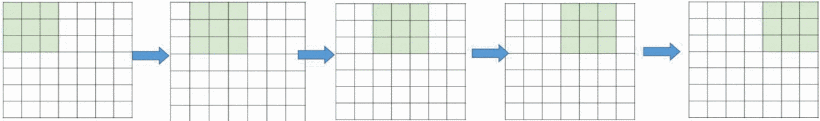
\includegraphics[width=0.7\textwidth]{images/CNN/fig_Stride.png}
            \caption{Esempio di movimento di un filtro $3 \times 3$ con stride 1. \cite{8308186}}
            \label{fig:Stride}
        \end{figure}
    
        \begin{figure}[h]
            \centering
            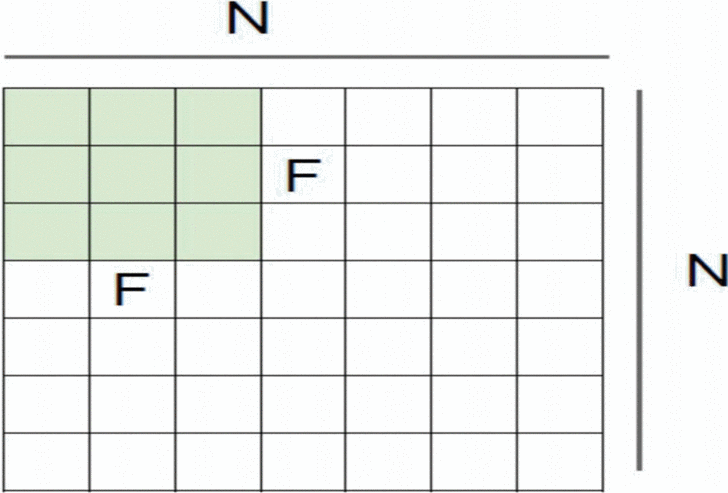
\includegraphics[width=0.7\textwidth]{images/CNN/fig_Stride2.png}
            \caption{Risultato dell'applicazione dello stride. \cite{8308186}}
            \label{fig:Stride2}
        \end{figure}

        \item[Padding] Uno degli svantaggi della fase di convoluzione è la perdita di informazioni che
        potrebbero esistere sul bordo dell'immagine, poiché durante la convoluzione i pixel del bordo sono 
        visti ed usati meno volte rispetto a quelli del centro, dato che il filtro li osserva solo quando 
        si muove attraverso l'immagine. Un metodo molto semplice ma efficace per risolvere il problema, è 
        usare zero-padding. L'altro vantaggio di zero-padding è quello di gestire la dimensione dell'output. 
        Per esempio, in Figura \ref{fig:Stride}, con $N=7$ e $F=3$ e stride 1, l'uscita sarà $5 \times 5$ 
        (che si restringe da un ingresso $7 \times 7$). Tuttavia, aggiungendo uno zero-padding, l'output 
        sarà $7 \times 7$, che è esattamente lo stesso dell'input originale (il valore attuale di $N$ 
        diventa 9, usata nella (1). L'equazione modificata che include zero-padding è la (2).
        \[ O=1+ \frac{N+2P-F}{S} \tag{2} \]
        dove $P$ è il numero dei livelli di riempimento applicati dallo zero-paddding (ad esempio $P=1$ in
        Figura \ref{fig:Padding}). Questa idea di riempimento ci aiuta a impedire che la dimensione dell'uscita
        di rete si restringa con la profondità. Pertanto, è possibile avere un numero qualsiasi di reti 
        convoluzionali profonde \cite{o2015introduction}.
    \end{description}

       \begin{figure}[h]
           \centering
           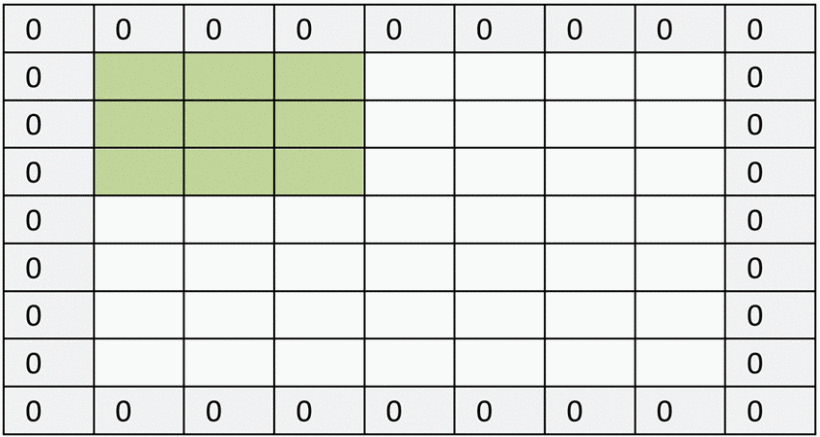
\includegraphics[width=0.7\textwidth]{images/CNN/fig_Padding.png}
           \caption{Effetto dello zero padding sull'immagine di input. \cite{8308186}}
           \label{fig:Padding}
       \end{figure}

    \begin{figure}[h]
        \centering
        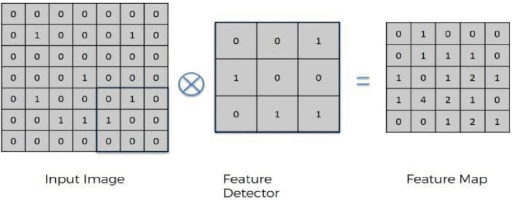
\includegraphics[width=0.7\textwidth]{images/ConvLayer_resize.png}
        \caption{Funzionamento della convoluzione \cite{9077735}}
        \label{fig:ConvKernel}
    \end{figure}
    
    \begin{figure}[h]
        \centering
        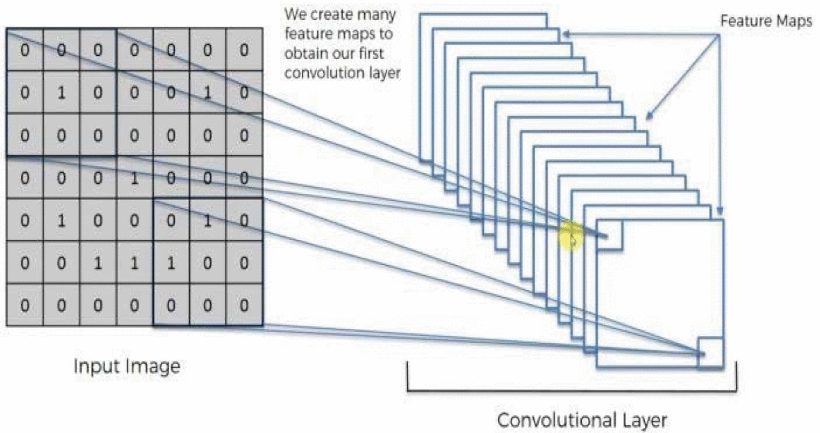
\includegraphics[width=0.7\textwidth]{images/CNN/ConvsLayer.png}
        \caption{Layer Convoluzionale \cite{9077735}}
        \label{fig:ConvLayer}
    \end{figure}
    \item[Pooling Layer] Il pooling è un passo importante per ridurre ulteriormente le dimensioni della mappa di
    attivazione, mantenendo solo le caratteristiche importanti e riducendo l'invarianza spaziale. Questo a sua 
    volta riduce il numero di caratteristiche apprendibili dal modello. Ciò aiuta a risolvere il problema del
    sovradimensionamento. Il pooling consente alla CNN di incorporare tutte le diverse dimensioni di un'immagine 
    in modo che la rete riconosca con successo l'oggetto dato anche se la sua forma è inclinata o è presente con
    un'angolazione diversa. 
    Ci sono vari tipi di pooling come il Max Pooling, l'Average Pooling, lo Stochastic Pooling e lo Spatial Pyramid
    Pooling. Tra questi, il più popolare è il Max Pooling che prende il valore più alto da ogni sub matrice della mappa 
    di attivazione e forma una matrice separata. In questo modo si assicura che le caratteristiche apprendibili
    rimangano limitate nel numero, preservando allo stesso tempo le caratteristiche chiave di qualsiasi immagine. 
    Il Max Pooling è solitamente fatto usando un filtro $2 \times 2$. La Figura \ref{fig:PoolLayer} mostra il
    funzionamento di tale layer.  
    \begin{figure}[h!]
        \centering
        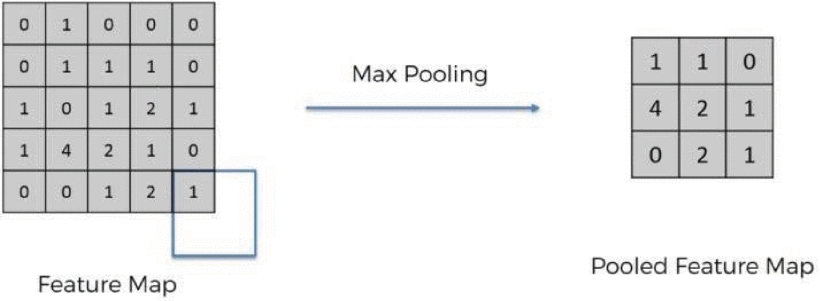
\includegraphics[width=0.7\textwidth]{images/PoolLayer.png}
        \caption{Applicazione Max Pooling \cite{9077735}}
        \label{fig:PoolLayer}
    \end{figure}
    \item[Batch Normalization layer] La Batch Normalization (BatchNorm) \cite{ioffe2015batch,9077735} è stata
    probabilmente una delle innovazioni architetturali di maggior successo nel deep learning e anche se la sua 
    efficacia è indiscutibile, non abbiamo una ferma comprensione del perché questo è il caso. In generale, 
    BatchNorm è un meccanismo che mira a stabilizzare la distribuzione (su un mini lotto) di input ad un
    determinato livello di rete durante l'addestramento. Ciò si ottiene aumentando la rete con strati aggiuntivi 
    che impostano i primi due momenti (media e varianza) della distribuzione di ciascuna attivazione rispettivamente 
    a $0$ (zero) e $1$ (uno). Poi, gli ingressi normalizzati batch sono in genere anche in scala e spostati sulla 
    base di parametri addestrabili per preservare l'espressività del modello. Questa normalizzazione viene applicata
    prima della non-linearità del layer precedente. Una delle motivazioni chiave per lo sviluppo di BatchNorm è 
    stata la riduzione del cosiddetto Spostamento Covariato Interno (Internal Covariate Shift).
    Questa riduzione è stata ampiamente considerata come il fulcro del successo di BatchNorm. Ioffe e Szegedy
    \cite{ioffe2015batch} descrivono l'ICS come "il fenomeno in cui la distribuzione degli input a un livello 
    della rete cambia a causa di un aggiornamento dei parametri dei livelli precedenti". Questo cambiamento porta 
    ad un costante spostamento del problema di formazione di base e si ritiene quindi che abbia un
    effetto negativo sul processo di training.
    \item[Drop-out Layer] Drop-out \cite{hinton2012improving} è un metodo per regolarizzare le reti neurali, 
    proposto per evitare l'over-fitting. È un metodo di regolarizzazione\footnote{Un metodo di regolarizzazione 
    è spesso formalmente definito come un metodo di inversione a seconda di un singolo parametro reale $\alpha \geq 0$
    che produce una famiglia di soluzioni approssimative $f(\alpha)$ con le seguenti due proprietà: 
    in primo luogo, per $\alpha$ grande abbastanza la soluzione regolarizzata $f(\alpha)$ è stabile a fronte di
    perturbazioni o rumore nei dati (a differenza della soluzione generalizzata) e, in secondo luogo, per $\alpha$ 
    che va a zero è recuperata la soluzione generalizzata non regolarizzata: $f(\alpha) = f() + \alpha \to 0$} 
    che imposta stocasticamente a zero le attivazioni delle unità nascoste per ogni caso di addestramento al momento
    della fase di training. 
    Questo interrompe il co-adattamento dei rilevatori di funzionalità poiché le unità degli strati nascosti 
    selezionati dal drop-out non possono influenzare le restanti unità. Un altro modo per interpretare il drop-out 
    è che produce una forma molto efficiente di media del modello in cui il numero di modelli addestrati è 
    esponenziale in quello delle unità, e questi modelli condividono gli stessi parametri. Il drop-out ha anche
    ispirato altri metodi stocastici come lo Stochastic Pooling \cite{zeiler2013stochastic} e 
    DropConnect \cite{wan2013regularization}. 
    Anche se il Drop-out è noto per funzionare bene in layer fully connected di reti neurali convoluzionali il 
    suo effetto non è stato ancora ben documentato \cite{wan2013regularization, zeiler2013stochastic,
    krizhevsky2017imagenet}.
    Il Drop-out è una nuova tecnica di regolarizzazione che è stata più recentemente impiegata nel deep learning. 
    È simile al bagging \cite{breiman1996bagging}, in cui un insieme di modelli sono addestrati su diversi sottoinsiemi
    degli stessi dati di allenamento. Al momento della prova, le previsioni dei diversi modelli sono mediate insieme.
    Nel bagging, ogni modello ha parametri indipendenti e tutti i membri sarebbero addestrati individualmente. 
    Nel caso di formazione tramite drop-out, ci sono esponenzialmente molti modelli eventualmente da
    addestrare ma non lo sono tutti in maniera palese, poiché questi ultimi condividono gli stessi parametri. 
    In realtà, il numero di modelli addestrati tramite drop-out non è più grande di $\gamma \times \epsilon$, 
    dove $\gamma$ è il numero di esempi di formazione, ed $\epsilon$ è il numero di epoche usate nel training. 
    Questo è molto più piccolo del numero di modelli eventualmente addestrati che è pari a $2^n$ 
    (dove $n$ è il numero di unità nascoste in una rete neurale feed-forward). Pertanto, la stragrande maggioranza 
    dei modelli non sono esplicitamente addestrati al momento della formazione.
    \item[Fully Connected Layer] Questo è il layer che viene utilizzato alla fine della rete neurale. 
    Generalmente la matrice dei pesi viene appiattita prima di essere passata ai neuroni. È difficile seguire i 
    dati dopo questo punto a causa della presenza di molte unità nascoste con peso variabile all'uscita di ogni 
    neurone. Tutto il ragionamento e il calcolo sui dati ed il raggiungimento di una target class associato al 
    nostro input, viene delegato a questa tipologia di layer.
\end{description}

\subsubsection{Funzioni d'attivazione}~\newline
\label{subsubsec:act_func}
Le CNN possono sfruttare diverse funzioni di attivazione per esprimere funzioni complesse. Simile alla funzione del
modello del neurone del cervello umano, la funzione di attivazione qui è un'unità che determina quale informazione
dovrebbe essere trasmessa al neurone seguente.
Ogni neurone nella rete neurale accetta il valore di uscita dei neuroni dal livello precedente come input e passa il
valore elaborato al livello successivo.
In una rete neurale multilayer, la funzione di attivazione è posta tra due layer e la struttura 
è mostrata nella figura \ref{fig:activation_func}.
\begin{figure}[h!]
    \centering
    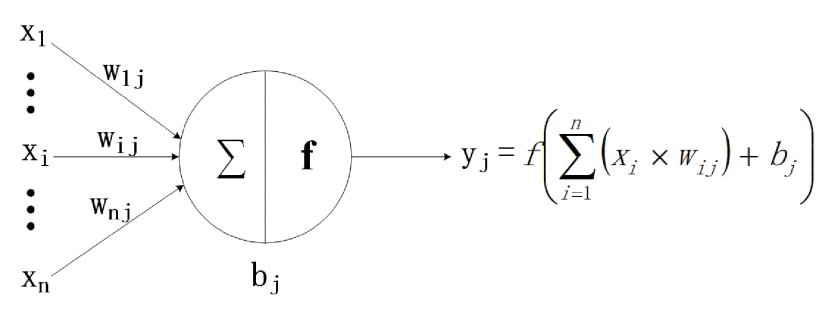
\includegraphics[width=\textwidth]{images/activaiton_func.png}
    \caption{Diagramma generale sulle funzioni d'attivazione \cite{9451544}}
    \label{fig:activation_func}
\end{figure}
In Figura \ref{fig:activation_func} , $x_{i}$ rappresenta la funzione di input; $n$ sono le caratteristiche in input 
al neurone $j$ allo stesso tempo; $W_{ij}$ rappresenta il valore di peso della connessione tra la funzione di input
$x_{i}$ e il neurone $j$; $b_{j}$ rappresenta lo stato interno del neurone $j$, che è il valore di bias; 
e $y_{j}$ è l'uscita del neurone $j$. $f()$ è la funzione di attivazione, che può essere la funzione sigmoide, 
la funzione Tanh \cite{726791} o l'unità lineare rettificata (ReLU) \cite{nair2010rectified}.
Se non viene utilizzata una funzione di attivazione o viene utilizzata una funzione lineare, l'input di ciascun 
livello sarà una funzione lineare dell'output del livello precedente. In questo caso, He et al. \cite{he2015delving}
dimostrano che non importa quanti layer ha la rete neurale, l'output sarà sempre una combinazione lineare dell'input, 
il che significa che i livelli nascosti non hanno effetto. Questa situazione rappresenta il modello del 
perceptron \cite{rosenblatt1958perceptron, rosenblatt1961principles}, che ha capacità di apprendimento limitata. 
Per questo motivo, le funzioni non lineari sono introdotte come funzioni di attivazione. Teoricamente, reti 
neurali profonde con funzioni di attivazione non lineari possono approssimare qualsiasi funzione, il che 
migliora notevolmente la capacità delle reti neurali di adattarsi ai dati.
La funzione sigmoide è una delle più tipiche funzioni di attivazione non lineari con una forma S complessiva (
vedere Figura \ref{fig:activation_function}(a)). 
Quando il valore $x$ si avvicina a $0$, il gradiente diventa più ripido. La funzione sigmoide può mappare un 
numero reale nell'intervallo $(0, 1)$, pertanto, può essere utilizzata per problemi di classificazione binaria. 
Inoltre, i modelli Senet \cite{hu2018squeeze} e MobileNet v3 \cite{howard2019searching} devono trasformare il 
valore di uscita di ogni layer in $(0, 1)$ per poter usare il loro meccanismo di attenzione. 
In questo contesto la sigmoide è la funzione più appropriata da implementare.
Diversamente dalla sigmoide, la funzione Tanh \cite{726791} (vedere Figura \ref{fig:activation_function}(b)) 
può mappare un numero reale nel range $(-1, 1)$. Poiché il valore medio dell'output di Tanh è $0$, può raggiungere 
una sorta di normalizzazione. Questo rende l'apprendimento di nuove complessità più facili per lo
strato successivo.
Oltre Tanh, esiste anche ReLU \cite{nair2010rectified} (vedere Figura \ref{fig:activation_function}(c)) che 
risulta essere un'altra funzione di attivazione efficace. 
Quando $x$ è inferiore a $0$, il suo valore di funzione è $0$; quando $x$ è maggiore o uguale a $0$, il suo valore 
di funzione è $x$ stesso. 
Rispetto alla funzione sigmoide e alla funzione Tanh, un vantaggio significativo dell'utilizzo della funzione ReLU è che 
può accelerare l'apprendimento. Sigmoide e Tanh mentre calcolano i derivati coinvolgono nel calcolo una funzione
esponenziale che include la divisione.
Il derivato di ReLU, invece, è una costante. Inoltre, nella funzione sigmoide e Tanh, se il valore di $x$ è troppo
grande o troppo piccolo, il gradiente della funzione è piccolo, il che può far convergere lentamente la funzione. 
Tuttavia, quando $x$ è inferiore a $0$, il derivato di ReLU è $0$, e quando $x$ è maggiore di $0$, la derivata è $1$;
quindi, si può ottenere un effetto di convergenza ideale. AlexNet \cite{krizhevsky2017imagenet}, il miglior modello 
in ILSVRC-2012, utilizza ReLU come funzione di attivazione del modello basato su CNN perché mitiga il problema della
scomparsa del gradiente quando la rete è profonda e verifica che l'uso di ReLU superi il sigma nelle reti profonde.

\begin{figure}[h!]
    \centering
    \subfloat[][]{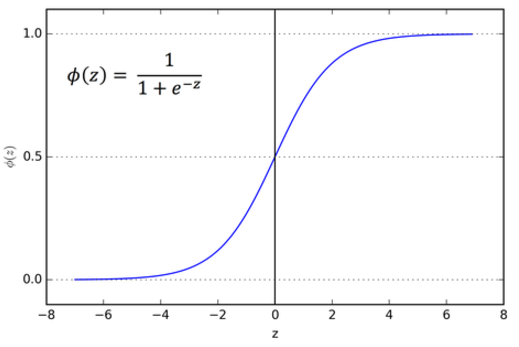
\includegraphics[scale=0.6]{images/ActivationFunction/sigmoid_function.png}} \hfill % 1
		\subfloat[][]{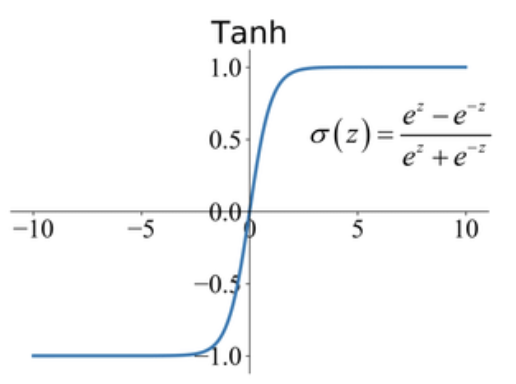
\includegraphics[scale=0.6]{images/ActivationFunction/Tanh_function.png}} \hfill % 2
		\subfloat[][]{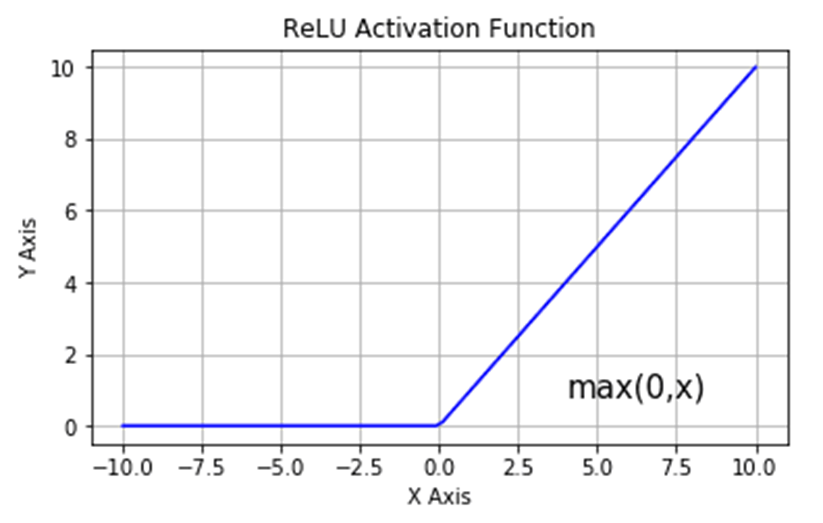
\includegraphics[scale=0.6]{images/ActivationFunction/ReLU_function.png}} \hfill % 3
    \caption{Esempi di funzioni d'attivazione: (a) Sigmoid, (b) Tanh, (c) ReLU}
    \label{fig:activation_function}
\end{figure}

Sulla base della discussione precedente, notiamo che ReLU non include il limite superiore. In pratica, 
possiamo impostare un limite superiore, come ReLU6 \cite{krizhevsky2010convolutional}.

\begin{figure}
    \centering
    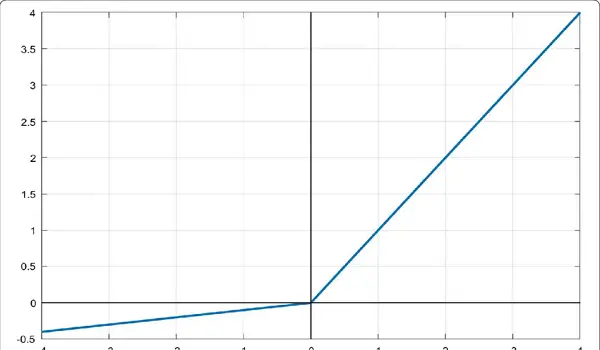
\includegraphics[width=0.7\textwidth]{images/leaky-ReLU-activation-function-new.png}
    \caption{La funzione Leaky ReLU}
    \label{fig:leaky_relu}
\end{figure}
Tuttavia un difetto di ReLU è che, quando $x$ è minore di $0$, il gradiente di ReLU è $0$. Ciò significa che 
l'errore retropropagato verrà moltiplicato per $0$, con il risultato che non verrà passato alcun errore al livello
precedente.
In questo scenario, i neuroni possono essere considerati inattivati o morti.
Pertanto, vengono proposte alcune versioni migliorate. Un esempio è Leaky ReLU (Figura \ref{fig:leaky_relu}) che riesce 
a ridurre l'inattivazione dei neuroni.
Quando $x$ è minore di $0$, l'errore retropropagato è $x/a$, invece di zero, dove $a$ è un parametro fisso
nell'intervallo $(1, +\infty)$.

\subsubsection{Funzioni di perdita}~\newline
\label{subsubsec:loss}
La funzione di perdita o la funzione di costo è sfruttata per calcolare la distanza fra il valore previsto ed il 
valore reale. La funzione di perdita è usata solitamente come criterio imparante del problema di ottimizzazione. 
La funzione di perdita può essere utilizzata con CNN per affrontare i problemi di regressione e i problemi di
classificazione, il cui obiettivo è quello di minimizzare la funzione stessa. Le funzioni di perdita comunemente usate
includono l'errore assoluto medio (MAE), l'errore quadratico medio (MSE), l'entropia trasversale e così via. 
Nelle CNN, ci sono molte funzioni di perdita da gestire quando si tratta di un task di classificazione. La più
conosciuta ed usata è la Cross-Entropy, che è usata per valutare la differenza tra la distribuzione di probabilità
ottenuta dall'allenamento corrente e la distribuzione effettiva. 
Questa funzione confronta la probabilità prevista con il valore di uscita effettivo ($0$ o $1$) in ogni classe 
e calcola il valore di penalità in base alla distanza da loro. La penalità è logaritmica, pertanto, la funzione 
fornisce una penalità minore ($0.1$ o $0.2$) per differenze più piccole tra le due distribuzioni e una penalità 
più grande ($0.9$ o $1.0$) per differenze più grandi.
La Cross-Entropy loss function è anche chiamata perdita di Softmax, poiché viene usata nelle reti convoluzionali 
in combinazione con un layer Softmax.
Ad esempio, AlexNet \cite{krizhevsky2017imagenet}, Inception v1 \cite{szegedy2015going} e Resnet \cite{he2016deep}
utilizzano la Cross-Entropy loss function come funzione di perdita nei loro articoli originali e ciò li ha aiutati 
a raggiungere risultati all'avanguardia. Tuttavia, la Cross-Entropy loss function ha alcuni difetti: essa si 
preoccupa solo della correttezza della classificazione ma non del grado di compattezza all'interno della stessa
classe o del margine tra classi diverse. 
Una delle varianti della Cross-Entropy è la Large-Margin Softmax loss \cite{liu2016large}. Lo scopo di questa 
funzione è di massimizzare la densità interna tra campioni di una stessa classe e massimizzare la distanza tra 
classi diverse. 
La Large-Margin Softmax loss aggiunge un margine tra classi diverse e introduce la regolarità di tale margine 
attraverso l'angolo della matrice del peso di vincolo. Tale funzione è stata utilizzata per face recognition 
\cite{liu2016large}, emotion recognition \cite{tan2017group}, speaker verification \cite{liu2019large}, e così via.

\subsubsection{Ottimizzatori}~\newline
\label{subsubsec:optimizer}
Nelle CNN, spesso abbiamo bisogno di ottimizzare le funzioni non convesse. I metodi matematici richiedono un'enorme
potenza di calcolo, pertanto, gli ottimizzatori vengono utilizzati nel processo di allenamento per ridurre al minimo 
la funzione di perdita e per ottenere parametri di rete ottimali in un tempo accettabile. Gli algoritmi di
ottimizzazione comuni includono momentum, Root-mean-square prop (RMSprop), stima del momento adattivo (Adam), e
così via. Ciascuno dei precedenti algoritmi si basa sulla discesa del gradiente e ne esistono tre tipi che si possono
utilizzare per allenare i modelli di CNN:
\begin{enumerate}
    \item Batch Gradient Descent (BGD)
    \item Stochastic Gradient Descent (SGD)
    \item mini-BGD (MBGD)
\end{enumerate}
Il BGD indica che un intero lotto di dati deve essere calcolato per ottenere un gradiente per ogni aggiornamento al
fine di garantire la convergenza all'ottimo globale del piano convesso e all'ottimo locale del piano non convesso.
Tuttavia, BGD è troppo lento da usare perché deve essere calcolato il gradiente medio dei campioni interi del lotto.
Inoltre, può essere difficile per i dati che non sono adatti per il calcolo in memoria. BGD, quindi, è difficilmente
utilizzato nella pratica nella formazione di modelli basati su CNN. Al contrario, SGD utilizza un solo
campione per ogni aggiornamento. È evidente che il tempo di SGD per ogni aggiornamento è notevolmente inferiore 
rispetto a BGD perché soltanto un gradiente del campione totale viene usato per il calcolo. In questo caso, SGD è 
adatto per l'apprendimento online \cite{saad1999line}. Tuttavia, SGD è rapidamente aggiornato con varianza elevata 
e ciò causa una forte oscillazione nella funzione di perdita.
Da un lato, l'oscillazione del calcolo può far saltare il calcolo del gradiente dall'ottimo locale e infine 
raggiungere un punto migliore.
D'altra parte, SGD non può mai convergere a causa dell'oscillazione infinita. In termini di tasso di convergenza,
supponendo che la deviazione standard di ciascun campione per la distribuzione reale sia $\sigma$, la deviazione
standard di $n$ campioni è $\frac{\sigma}{\sqrt{n - 1}}$. 
Quando usiamo i campioni per stimare il gradiente, un campione introduce una deviazione standard pari a $\sigma$,
ma usandone $n$ ciò non fa diminuire linearmente la deviazione standard. L'unica cosa che aumenta è la quantità 
di calcolo sugli $n$ campioni e l'aumento è lineare. 
Sulla premessa di questa stessa quantità di calcolo, la velocità di convergenza dell'utilizzo dell'intero set di
campioni è molto più lenta rispetto all'utilizzo di un piccolo numero di campioni. In altre parole, per convergere
nello stesso punto ottimale, quando si utilizza l'intero set di allenamento, anche se il numero di iterazioni è 
piccolo, il tempo di ogni iterazione è lungo. Quindi, il costo totale di tempo è maggiore rispetto 
ad un piccolo numero di campioni per più iterazioni multiple.

Teoricamente, quanto affermato prima è vero, ossia minore è il numero di campioni, più veloce sarà il tasso 
di convergenza quando si utilizza una CPU single-core. Tuttavia, quando si utilizzano le GPU per l'addestramento, 
a causa del gran numero di core ed all'eccellente capacità di calcolo parallelo della GPU, ci vuole lo stesso 
tempo sia per calcolare un campione sia per calcolarne decine o centinaia. 
Pertanto, nella pratica ingegneristica basata su BGD e SGD, MBGD è stato proposto e utilizzato frequentemente. 
Esso combina i vantaggi di BGD e SGD e la dimensione del batch dipende dalla memoria della GPU e dal core di calcolo. 
MBGD utilizza un piccolo lotto di campioni per ogni aggiornamento in modo che possa non solo eseguire la discesa 
del gradiente in modo più efficiente di BGD, ma anche ridurre la varianza rendendo la convergenza più stabile.

Molti modelli classici della CNN utilizzano MGBD per addestrare le loro reti, come AlexNet
\cite{krizhevsky2017imagenet}, VGG \cite{simonyan2014very}, inception v2 \cite{szegedy2015going}, 
Resnet \cite{krizhevsky2017imagenet} e DenseNet \cite{huang2017densely}.
È stata inoltre utilizzata in FaceNet \cite{schroff2015facenet}, DeepID \cite{sun2014deep} e DeepID2 \cite{sun2014deeps}.
Sulla base di MBGD, sono stati proposti una serie di algoritmi efficaci per l'ottimizzazione per accelerare il 
processo di formazione del modello. Qui di seguito mostriamo alcuni ottimizzatori che si basano MBDG:

\begin{itemize}
    \item  L'algoritmo di Adagrad \cite{duchi2011adaptive} è un altro algoritmo di ottimizzazione basato sui gradienti.
           Può adattare dinamicamente il learning rate ai parametri delle rete, cioè esegue piccoli aggiornamenti 
           (se ad esempio, sussiste un basso learning rate) per caratteristiche che si mostrano con alta frequenza 
           ed esegue aggiornamenti più ampi (cioè, con un alto learning rate) per quelle non frequenti. 
           Pertanto, è adatto per l'elaborazione di dati sparsi. Uno dei principali vantaggi di Adagrad è che non è 
           necessario regolare manualmente il tasso di apprendimento. 
           Nella maggior parte dei casi, si usa solo $0.01$ come learning rate predefinito \cite{ma2018shufflenet}. 
           Ad esempio FaceNet \cite{schroff2015facenet} utilizza Adagrad come ottimizzatore in allenamento.

    \item L'algoritmo di Adadelta \cite{zeiler2012adadelta}, che è un'estensione dell'Adagrad, è progettato per 
          ridurre il suo learning rate come una funzione monotona descrescente.
          Non si limita ad accumulare tutti i gradienti al quadrato, ma imposta una finestra di dimensioni fisse 
          per limitare il numero di gradienti al quadrato accumulati. Allo stesso tempo, la somma dei gradienti 
          è definita ricorsivamente come la media di decadimento di tutti i gradienti precedentemente quadrati,
          piuttosto che memorizzare direttamente i gradienti precedentemente quadrati. L'algoritmo Adadelta è 
          sfruttato in molti compiti come speech recognition e sentence classification \cite{chorowski2015attention,
          kim-2014-convolutional}.

    \item L'algoritmo RMSprop \cite{hinton2012neural} è progettato per risolvere il problema del tasso di 
          apprendimento radicalmente decrescente nell'algoritmo Adagrad. MobileNet \cite{howard2017mobilenets}, 
          versione iniziale v3 \cite{szegedy2016rethinking} e versione iniziale v4 \cite{szegedy2017inception} 
          hanno ottenuto i migliori modelli utilizzando RMSprop.

    \item Un altro ottimizzatore utilizzato di frequente è la stima adattiva del momento (Adam) \cite{kingma2014adam}. 
          È essenzialmente un algoritmo formato combinando la quantità di moto con l'RMSprop. Adam memorizza 
          sia la media di decadimento esponenziale dei gradienti quadrati passati, come l'algoritmo Adadelta, 
          sia la media di decadimento esponenziale medio dei gradienti passati, come l'algoritmo di quantità di moto. 
          La pratica ha dimostrato che l'algoritmo Adam funziona bene su molti problemi ed è applicabile a molte 
          strutture diverse di CNN \cite{sharma2015action,van2018predicting}.

          L'algoritmo AdaMax \cite{kingma2014adam} è una variante di Adam che semplifica l'intervallo di confine 
          del tasso di apprendimento ed è stato utilizzato per addestrare i modelli CNN di \cite{van2018predicting} e
          \cite{niklaus2017video}.

          La stima di Adam accelerata da Nesterov (Nadam) \cite{dozat2016incorporating} è una combinazione di Adam 
          e NAG. Nadam ha un vincolo più forte sul tasso di apprendimento e un impatto diretto sull'aggiornamento 
          del gradiente. Nadam è utilizzato in molti compiti come la classificazione del livello del suono in un 
          luogo \cite{nguyen2018convolutional,schindler2018multi}.
\end{itemize}

\subsubsection{Hyperparameter tuning}~\newline
Quando si costruisce una CNN, oltre a selezionare la funzione di attivazione, la funzione di perdita e l'ottimizzatore,
dobbiamo anche regolare molti altri iperparametri che influiscono notevolmente sulle prestazioni del modello. Come è
noto, non esiste un insieme fisso di iperparametri in grado di garantire una soluzione ottimale per tutto il tempo. 
Per cui, un insieme di esperienze e buone regole pratiche sono significative durante l'hyperparameter tuning. 
Un modello di deep neural network (DNN) apprende i valori appropriati delle sue variabili di configurazione, 
cioè i pesi di connessione e il bias, dai dati di allenamento e, tali variabili, sono chiamate parametri
\cite{nasrabadi2007pattern}. 
Il processo di determinazione dei loro valori dai dati è noto come formazione o apprendimento del modello.
Tuttavia, ci sono alcuni parametri di alto livello noti come "iperparametri" i cui valori non possono essere 
appresi dai dati \cite{bergstra2011algorithms}. Alcuni degli iperparametri importanti per le architetture DNN 
includono il numero di layer, il numero di nodi, il tasso di apprendimento, il tasso di regolarizzazione, 
la funzione di perdita, la funzione di attivazione, il metodo di ottimizzazione, il metodo di valutazione, ecc.
L'addestramento di una DNN è un processo relativamente ingombrante poiché queste ultime devono essere
addestrate con una grande quantità di dati per imparare i loro parametri con precisione \cite{lecun2015deep,
schmidhuber2015deep}. 
Anche una singola istanza del problema di formazione della rete neurale potrebbe richiedere giorni o addirittura
settimane per allenarsi. Ciò influenza anche le reti neurali convoluzionali (CNN) distribuite per riconoscere le
immagini e video \cite{pmlr-v9-glorot10a}.
Quando la CNN tenta di riconfigurare i suoi parametri dopo l'introduzione di piccoli rumori, si rischia 
l'over-fitting e il rallentamento della convergenza del modello \cite{7536654}. Allo stesso modo, 
l'addestramento delle reti neurali ricorrenti (RNN) è un compito difficile poiché hanno un'architettura 
complessa e soffrono di problemi di gradienti che svaniscono \cite{Pascanu2013}.
Le prestazioni di formazione delle DNN e la loro struttura dipendono fortemente dalle scelte dei valori 
degli iperparametri \cite{Dobslaw2010APF}.
Perciò, decidere i valori ottimali degli iperparametri è essenziale per esprimere il massimo potenziale dei modelli 
DNN \cite{7536654}. 
La Tabella \ref{tab:Hyper_tab} a pagina \pageref{tab:Hyper_tab} mostra come alcuni iperparametri comuni influenzano le prestazioni dei modelli.
\begin{table}[hpbt!]
    \centering
    \caption{Iperparametri più comuni}
    \footnotesize
    \begin{tabular}{>{\bfseries}lp{0.50\textwidth}l}
    \toprule
        Iperparametri & Descrizione \\
        \midrule
         Learning rates &  Il tasso di apprendimento si riferisce alla dimensione del passo di aggiornamento dei pesi di
         rete. Può essere costante o variabile. Come accennato nella sottosezione Ottimizzatori
         \ref{subsubsec:optimizer}, gli algoritmi di ottimizzazione determinano diversi tassi di apprendimento. Per
         rendere la discesa in pendenza migliore, il valore della velocità di apprendimento dovrebbe essere impostato 
         in un intervallo appropriato. Se la velocità di apprendimento è troppo piccola, la velocità di convergenza 
         sarà lenta; se è troppo grande, i parametri oscilleranno avanti e indietro su entrambi i lati della soluzione
         ottimale. \\
         \midrule
         Epoch & L'epoca si riferisce al numero di volte che tutto l'insieme di addestramento è dato in input 
         alla rete neurale per il training. Quando il divario di accuratezza fra l'insieme di addestramento e l'insieme
         di convalida è piccolo, l'epoca corrente è considerata appropriata. Altrimenti, se il divario diminuisce,
         significa che l'epoca è troppo piccola, con conseguente under-fitting; se il divario aumenta, l'epoca è 
         troppo grande, con conseguente over-fitting.\\  
         \midrule
         Mini-batch size & La dimensione del lotto mini è il numero di campioni inviati al modello in ogni allenamento.
         Nel processo di ottimizzazione della rete, avere la dimensione del batch troppo piccola significa che il numero
         di campioni immessi nella rete è troppo piccolo, cioè non rappresentativo, e il rumore aumenta di conseguenza,
         il che rende la convergenza della rete molto difficoltosa. La dimensione del lotto troppo grande rende la
         direzione del gradiente quasi stabile e ciò rende la discesa del gradiente rapida verso un punto ottimale
         locale o sella locale.\\
         \midrule
         Number of conv layers e conv kernels & Ogni livello Conv di solito contiene caratteristiche di livello diverso.
         Gli strati superficiali possono rilevare le caratteristiche dei bordi, le caratteristiche locali e altre
         caratteristiche a basso livello dell'immagine, mentre gli strati profondi possono rilevare le caratteristiche
         globali. Di solito, le reti con più livelli e kernel hanno la capacità di rappresentare caratteristiche più
         complesse, ma nel frattempo, sono più difficili da addestrare. \\
         \midrule
         Size of conv kernels & Sulla premessa dello stesso campo ricettivo, più piccolo è il kernel di convoluzione,
         meno sono i parametri e meno complessità computazionale è richiesta. In particolare, quando la dimensione del
         kernel di convoluzione è maggiore di $1$, può aumentare il campo ricettivo. Se si usa il kernel di convolutione
         con dimensione pari, anche se il padding viene aggiunto simmetricamente, non possono essere mantenute invariate
         la dimensione della mappa delle caratteristiche di input e la dimensione della mappa delle caratteristiche di
         output .\\
         \bottomrule
    \end{tabular}
    \normalsize
    \label{tab:Hyper_tab}
\end{table}

\subsection{Generazione delle Heatmap}~\newline
Le heatmap sono generate sulla base dell'idea di Guided Grad-CAM \cite{selvaraju2017grad}. Come premessa bisogna usare
solo il dataset di training sulla rete CNN già addestrata, in seguito, per ogni campione di dati, si è riportato la
mappa di attivazione dell'ultimo layer convoluzionale durante il processo di forward passing.
Poi, attraverso il processo di backpropagation, abbiamo registrato i gradienti specifici dell'etichetta di ogni neurone
dell'ultimo layer convoluzionale. Questi gradienti rappresentano il contributo dei neuroni ai risultati della
classificazione. La Grad-CAM viene calcolata utilizzando una somma ponderata delle mappe di attivazione che viene 
poi ridimensionata alle dimensioni dell'input. Per migliorare ulteriormente l'accuratezza della localizzazione, i
gradienti del layer di input sono moltiplicati con la Grad-CAM, generando infine la Guided Grad-CAM per ciascun
campione, che può essere visualizzata come una heatmap. 
Successivamente, è stata calcolata la media di tutte le heatmap della stessa classe e, dopo la normalizzazione, sono
state ottenute le heatmap per ogni classe. L'intensità di ciascun pixel rappresenta il significance score del gene 
che corrisponde al contributo dato da quest'ultimo alla classificazione.
In realtà, questo processo di generazione delle heatmap potrebbe essere impiantato nell'addestramento della rete 
neurale convoluzionale poiché non influisce sul processo di addestramento e di test.
La computazione è, però, minore con il metodo a due fasi descritto precedentemente, poiché la Grad-CAM richiede che
tutti i campioni passino una sola volta attraverso la rete neurale.

\subsubsection{Gradient Classification Activation Map}~\newline
Un certo numero di opere precedenti hanno affermato che rappresentazioni più profonde in una CNN catturano costrutti
visivi di livello superiore \cite{bengio2013representation, mahendran2016visualizing}. Inoltre, le caratteristiche
convoluzionali mantengono naturalmente le informazioni spaziali che vengono perse nei layer fully connected, quindi
possiamo aspettarci che gli ultimi layer convoluzionali abbiano il miglior compromesso tra semantica di alto livello 
e informazioni spaziali dettagliate.
I neuroni in questi layer cercano nell'immagine informazioni semantiche specifiche della classe (ad esempio, parti di
oggetti). Grad-CAM usa le informazioni di gradiente che fluiscono nell'ultimo strato convoluzionale della CNN per 
capire l'importanza di ogni neurone per una decisione di interesse. Anche se la nostra tecnica è molto generica e 
può essere utilizzata per visualizzare qualsiasi attivazione in una rete profonda, in questo lavoro ci concentriamo
sulla spiegazione delle decisioni che la rete può prendere eventualmente.

Come mostrato in Figura \ref{fig:GuidedGCam} a pagina \ref{fig:GuidedGCam}, al fine di ottenere la mappa di
localizzazione classe-discriminante Grad-CAM del layer $L$ definita come 
$L_{\text{Grad}-\text{CAM}}^{c}\in \mathbb{R}^{u \times v}$ di larghezza $u$ e altezza $v$ per qualsiasi classe $c$, 
in primo luogo calcoliamo il gradiente del punteggio per la classe $c$, $y^{c}$ (prima del Softmax), rispetto alla 
mappa delle caratteristiche $A^{k}$ di uno strato convoluzionale,cioè  $\frac{\partial y^{c}}{\partial A^{k}}$. 
Questi gradienti che scorrono indietro sono raggruppati nella media globale per ottenere i pesi 
$\alpha^{c}_{k}$ dell'importanza dei neuroni:
\[
    \alpha_{k}^{c}=\overbrace{\frac{1}{Z}\sum_{i}\sum_{j}}^{\text{global average pooling}}
    \underbrace{\frac{\partial y^{c}}{\partial A_{ij}^{k}}}_{\text{gradients via backprop}}\tag{1}
\]

Questo peso $\alpha^{c}_{k}$ rappresenta una linearizzazione parziale della rete profonda a valle di $A$, e 
cattura l'importanza della mappa caratteristica $k$ per una classe target $c$.

Eseguiamo una combinazione ponderata di mappe di attivazione in avanti e applichiamo ReLU per ottenere:
\[
    L_{\text{Grad}-\text{CAM}}^{c}=ReLU\underbrace{\left(\sum_{k}\alpha_{k}^{c}A^{k}\right)}_{\text{linear
    combination}}\tag{2}
\]

Si noti che ciò comporta una heatmap grossolana delle stesse dimensioni delle mappe delle caratteristiche 
convoluzionali ($14 \times 14$  nel caso degli ultimi strati convoluzionali della rete VGG \cite{simonyan2014very} 
e AlexNet \cite{krizhevsky2017imagenet}). 
Gli studi di ablazione e più visualizzazioni di Grad-CAM possono essere trovati in \cite{selvaraju2016grad}. 
In generale, $y^{c}$ non deve essere il punteggio di classe prodotto da una classificazione di immagine tramite CNN.
Potrebbe essere un'attivazione differenziabile che include parole da una didascalia o la risposta a una domanda.

\subsubsection{Guided BackPropagation}~\newline
Parte del potere d'interpretazione visiva di Guided Grad-CAM è ottenuta utilizzando l'algoritmo di Guided
Backpropagation basato sul gradiente (GBP) \cite{springenberg2014striving}, che si concentra sui pixel rilevanti 
delle immagini, responsabili della previsione della tipologia tumorale, fornendo un punteggio di confidenza a 
ciascun pixel. L'algoritmo GBP esegue una propagazione in avanti attraverso il modello in cui l'input viene passato
attraverso la funzione di attivazione ReLU, come descritto nell'Equazione \ref{eq:3}. Qui l'input $z_{i}^{l}$
rappresenta il punteggio di attribuzione per ogni timestamp. In questo caso, l'ingresso $z_{i}^{l}$ rappresenta 
l'uscita dell'$i^{th}$ neurone dell'$l^{th}$ strato. Durante la propagazione all'indietro, le saliency map ottenute 
con il filtro di convoluzione passano solo i valori che sono stati positivi durante il passaggio in avanti e
tagliano il resto dei valori. Ciò è visibile nell'Equazione \ref{eq:4}. Il segnale di errore $E_{i}^{l+1}$ 
rappresenta l'errore proveniente dall'$i^{th}$ neurone dello strato $(l+1)^{th}$. Il GBP modifica la propagazione
all'indietro classica, aggiungendo un'ulteriore condizione: passano solo i valori che sono stati positivi durante 
la propagazione in avanti e all'indietro. Dunque, dato questo vincolo viene generato un nuovo segnale di errore che 
tiene conto sia di $z_{i}^{l}$ sia di $E_{i}^{l+1}$ prima di passare l'errore al livello precedente, come descritto
nell'Equazione \ref{eq:5}. Pertanto, il gradiente è guidato dall'input dello strato precedente e dal segnale di 
errore dello strato successivo. I gradienti retropropagati evidenziano solo i pixel che influenzano fortemente la
diagnosi sulla tipologia di coorte tumorale, mentre la retropropagazione convenzionale non maschera le voci
negative durante la propagazione all'indietro. Il GBP calcola la versione vincolata del gradiente rispetto all'input,
mantenendo costante la matrice dei pesi della rete $\theta$ e utilizzando ReLU. Essendo una tecnica interpretabile a
posteriori, GBP non influenza la capacità decisionale del modello.

\begin{gather*} 
z_{i}^{l+1}=ReLU(z_{i}^{l})=max(z_{i}^{l},\ 0)\tag{3} \label{eq:3} \\ 
E_{i}^{l}=E_{i}^{l+1}\ \forall\ (z_{i}^{l} > 0),\ where\ E_{i}^{l+1}= \frac{\delta z^{out}}{\delta z_{i}^{l+1}}\tag{4} \label{eq:4}\\ E_{i}^{l}=E_{i}^{l+1}\ \forall\ (z_{i}^{l} > 0)\ and\ (E_{i}^{l+1} > 0)\tag{5} \label{eq:5}\\
\end{gather*}

\subsubsection{Guided GradCam}~\newline
Mentre le visualizzazioni Grad-CAM sono class-discriminant e localizzano bene le regioni più rilevanti in un'immagine,
esse non hanno la capacità di mostrare l'importanza a grana fine come i metodi di visualizzazione gradient pixel-space
transformation (ad es. guided backpropagation e deconvolution).
Per esempio, in Figura \ref{fig:GuidedGCam} a pagina \pageref{fig:GuidedGCam}, si può notare come nell'immagine 
indicata con \textbf{Grad-CAM}, vengano facilmente localizzate le regioni rilevanti del gatto; tuttavia, non è chiaro
dalle basse risoluzioni della heatmap perché la rete prevede questa particolare istanza come "gatto tigre".
Al fine di combinare gli aspetti migliori di entrambi, si fondono entrambi questi metodi di visualizzazione, Guided
Backpropagation e Grad-CAM, tramite moltiplicazione puntiforme ($L_{Grad-CAM}^{c}$ prima di essere moltiplicata 
con i gradienti generati da GBP viene ridimensionata alla risoluzione dell'immagine di ingresso utilizzando
interpolazione bi-lineare). Nella Figura \ref{fig:GuidedGCam} si può notare nell'immagine etichettata come
\textbf{Guieded Grad-CAM} come la heatmap generata con il procedimento descritto in precedenza sia ad alta risoluzione
e classe discriminante (ossia quando la classe di interesse è "gatto tigre", oltre che identificare importanti
caratteristiche del "gatto tigre", come strisce, orecchie a punta e gli occhi mostra anche la corretta tipologia 
di animale, cioè "gatto tigre" e non un altra classe). 
La sostituzione di Guided Backpropagation con Deconvolution, in base a quanto descritto sopra, dà risultati simili. 
Di fatti in \cite{lyu2018deep} hanno constato, però, che Deconvolution aveva degli artefatti: un vincolo
sull'architettura della rete presa in analisi e che le visualizzazioni erano rumorose rispetto a Guided
Backpropagation che erano generalmente meno rumorose. Per tali motivi, quindi, viene scelta come tecnica di 
gradient pixel-space transformation, Guided Backpropagation al posto di Deconvolution.
 \begin{figure}[h]
            \centering
            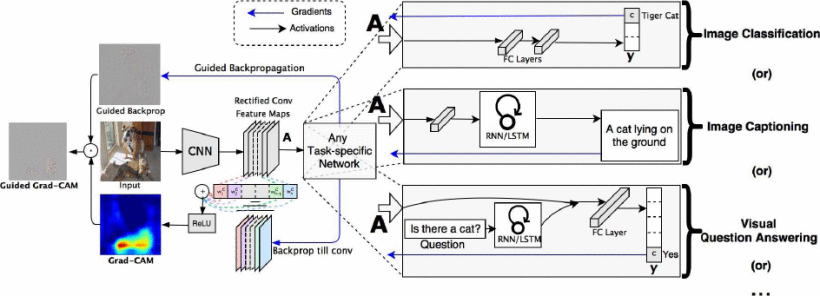
\includegraphics[width=0.9\textwidth]{images/Guided Grad-Cam/large_Guided_GradCam.png}
            \caption{Overview di Guided Grad CAM \cite{selvaraju2017grad}}
            \label{fig:GuidedGCam}
        \end{figure}
        
\subsection{Validazione}
I geni principali sono stati selezionati in base alla classifica dei significance score nelle heatmap. Abbiamo 
applicato l'analisi funzionale a questi top gene per dimostrare ulteriormente che i geni sono specifici per il tumore 
e che sono potenziali biomarker. 
Nella prima fase, abbiamo scelto i primi 400 geni più importanti di ciascun tipo di tumore per effettuare la pathway
analysis (analisi dei percorsi biologici), cercando di scoprire se i percorsi significativamente arricchiti
(significantly enriched pathway) sono correlati al tumore corrispondente. 

\subsubsection{Enchriment Pathway Analysis}~\newline
La Pathway Analysis (PA), nota anche come analisi di arricchimento funzionale, sta rapidamente diventando uno degli
strumenti più importanti della ricerca Omics\footnote{Con il termine OMICS si intendono tutte quelle scienze biologiche
il cui nome termina con il suffisso -omics, ad esempio genomics, transcriptomics, proteomics, metabolomics.}. 
Lo scopo principale degli strumenti di PA è di analizzare i dati ottenuti dalle tecnologie ad alta-capacità di
lavorazione, individuare i gruppi relativi ai geni legati alle alterazioni nei campioni di caso rispetto ad un 
campione di controllo. In questo modo, i metodi di PA cercano di superare il problema della dimensionalità 
introdotta dal dover interpretare grandi liste contenenti geni importanti, ma isolati dal contesto biologico, che
sono l'output principale dell'analisi dei dati ad alta-capacità di lavorazione prodotti dalla maggior parte delle
tecniche biologiche che si basano sull'analisi funzionale, come l'analisi di espressione differenziale. 
I metodi PA invece forniscono significato ai dati biologici sperimentali ad alto rendimento (High Troughput Biological
Data, in breve HTBD) facilitando così l'interpretazione e la successiva generazione di ipotesi. 
Ciò è stato ottenuto sulla base dell'accoppiamento delle conoscenze biologiche esistenti provenienti da banche dati 
con test statistici, analisi matematiche e algoritmi computazionali. I metodi di PA possiedono una vasta gamma 
di applicazioni nella ricerca fisiologica e biomedica. Questi metodi mirano ad aiutare il ricercatore a scoprire 
quali temi biologici, e quali biomolecole, sono cruciali per comprendere i fenomeni in studio, dato gli HTBD
analizzati. A sua volta, gli indizi che fornisce una PA consentono al ricercatore di generare nuove ipotesi, progettare
esperimenti successivi e convalidare ulteriormente i loro risultati. I metodi di PA hanno aiutato i ricercatori
nell'identificazione dei ruoli biologici dei geni candidati, selezionati per progettare nuove terapie per il cancro,
aggirando i danni collaterali alle cellule sane \cite{folger2011predicting}.
Ci sono diversi elementi necessari per eseguire una PA. Prima di tutto, sono necessari dati quantitativi rappresentativi
della biologia cellulare che sono generati con l'uso delle tecnologie di Omics come: RNA-microarrays, tandem mass
spectrometry e RNA-sequencing. 
In secondo luogo, un approccio in grado di analizzare una tale quantità sostanziale di dati è obbligatorio. 
La biologia dei sistemi è un campo di ricerca emergente che consente lo studio degli organismi viventi come sistemi,
opponendosi ad approcci riduzionisti \cite{hartwell1999murray, kitano2002computational}, utilizzando i dati Omics 
come input principale delle sue analisi. In terzo luogo, le conoscenze biologiche molecolari memorizzate in basi 
di dati sono necessarie per l'analisi da eseguire, guidando i metodi PA per cercare le relazioni tra i dati 
Omics generati e temi biologici noti. Infine, il potere computazionale necessario per realizzare PA consiste
principalmente nella computazione necessaria ad eseguire il test statistico dei temi biologici vs. i dati, e 
alla complessità degli altri algoritmi matematici che cercano di estrarre le relazioni tra i dati e le conoscenze
precedenti. 
Un altro esempio è la determinazione della somiglianza e della diversità, a livello molecolare, tra gruppi di campioni,
come nel confronto tra linee cellulari e campioni tumorali \cite{heiser2012subtype}. Questo tipo di analisi può 
aiutare i ricercatori a comprendere i fenomeni di eterogeneità in diversi contesti di ricerca. Un altro esempio 
ancora è l'uso di metodi PA per esaminare la funzione biologica dei moduli genici. I ricercatori hanno
dovuto convalidare insiemi di geni pensati per essere correlati tra loro, come nell'analisi dei geni che fluttuano 
in risposta alle variazioni naturali, come le stagioni \cite{dopico2015widespread}. Anche se tutte queste 
applicazioni hanno avuto successo in obiettivi specifici, l'uso di metodi di PA può essere ampia e complessa come 
la creatività del loro utente. Gli sforzi nella strutturazione della conoscenza biologica sulle pathway hanno provocato 
la generazione delle basi di dati delle pathway (PDBs), anche denominate "basi di conoscenza," che condensano la
conoscenza biologica corrente delle interazioni molecolari nelle raccolte di dati delle pathway. I PDBs di 
solito recuperano e strutturano dati da fonti diverse. Generalmente, le prove sperimentali sono curate dalla 
letteratura e le analisi computazionali sono effettuate dal progetto stesso per inferire le funzioni possibili delle
biomolecole omologhe.
Inoltre, viene generalmente fatto un riferimento incrociato dei dati tra database simili. Ad esempio, le annotazioni 
del database Reactome \cite{vastrik2007reactome} sono curate manualmente dalla letteratura da biologi esperti in
collaborazione con il loro staff editoriale, e cross-referenced con diverse altre risorse, come letteratura primaria,
e altri PDBs correlati \cite{ogata1999kegg}. Aggiunte e correzioni ai PDBs sono effettuate
periodicamente, aumentando così la qualità e la copertura delle loro conoscenze biologiche.
Alcuni database sono in grado di aggiornare le proprie informazioni in modo frequente, per mantenere il passo con le
nuove scoperte. Ad esempio il database KEGG \cite{kanehisa1997database} aggiorna i suoi dati su base settimanale, ma
altri PDBs lo fanno meno spesso, come Gene Ontology \cite{dolinski2000gene}, che aggiorna i suoi dati su base mensile.
Tuttavia, alcuni PDBs non riescono ad aggiornare le loro informazioni in modo regolare, quindi diventano
obsoleti nel corso del tempo, eppure vengono utilizzati dagli utenti di strumenti di PA, quindi si suggerisce 
cautela nell'uso di dati PDB obsoleti.
Quando si esegue la PA è necessario considerare la qualità dei dati nei PDBs e, come ulteriore fattore, è necessario
considerare anche la copertura offerta dai PDBs.
Si tratta della proporzione di componenti biologici aggregati descritti in tutti i percorsi di un PDB rispetto a 
un elenco di riferimento di componenti. 
Ad esempio, uno dei più completi PDB pubblici compositi, Pathway Commons \cite{cerami2010pathway}, con le informazioni
aggregate di 22 PDBs, ha attualmente una copertura di 17.439 simboli genici sui 39.241 accettati, pari a circa 
il $45\%$ dei simboli totali dei registri ufficiali del Comitato per la nomenclatura del genoma HUGO\footnote{
Progetto approvato dal Comitato per la nomenclatura del genoma (HGNC)}. L'utilizzo delle informazioni più aggiornate 
e complete è importante per l'estrazione ottimale di informazioni dai dati sperimentali. Raggiungere questo obiettivo
non è solo un invito agli utenti a utilizzare i migliori PDB disponibili, ma è anche un invito ai
potenziali contributori a migliorare la copertura e la conoscenza contenuta nei database. La maggior parte delle 
banche dati pubbliche incoraggia sforzi di collaborazione aperti, con la corrispondente revisione dei dati condivisi.
Tutti questi miglioramenti nei PDBs porteranno, in conclusione, ad una più rapida scoperta della conoscenza e
ad una più rapida applicazione delle conoscenze biologiche. 